\documentclass[handout]{beamer}
%\documentclass{beamer}

\usepackage{beamerthemesplit} \usepackage{amsmath}
\usepackage{amssymb} \usepackage{graphicx} \usepackage{floatflt}
\usepackage{amsthm}
\usepackage{tikz}
\usetikzlibrary{matrix,arrows}
\usepackage{fancybox}
\usepackage{array}
%\newcolumntype{L}{>{\centering\arraybackslash}m{3.1cm}}
\usepackage{mathrsfs}
\usepackage{hyperref}
%\usepackage{chngcntr}
\usepackage{xcolor}
%\usepackage[left=2.5cm,top=2cm,right=2.5cm,bottom=2cm,head=.95cm,foot=.95cm]{geometry}
%\usepackage{bbding}
%\usepackage{pifont}
%%\usepackage{listofitems}
%\usepackage{stackengine}
%\stackMath
%\setstackgap{S}{1pt}
%\usepackage{wasysym}

\usepackage{graphicx}



\setbeamertemplate{theorems}[numbered]

%\usetheme{Berkeley}
\usetheme{Copenhagen}

\definecolor{uofsgreen}{rgb}{.125,.5,.55}
% \definecolor{uofsgreen}{rgb}{.125,.5,.25}
\usecolortheme[named=uofsgreen]{structure}
%\usecolortheme{owl}

\setbeamercolor{normal text}{fg=white,bg=black}



\title{Is your advice unethical?}

\author{Scott Atkinson}

\date{ }


\newtheorem*{thm}{Theorem}
\newtheorem*{prop}{Proposition} 
\newtheorem*{conj}{Conjecture}
\newtheorem*{lem}{Lemma}
\newtheorem*{cor}{Corollary}
\newtheorem*{fct}{Fact}
\newtheorem*{lemA}{Cross-terms lemma}
\newtheorem*{lemB}{$Y_1$-square lemma}


\theoremstyle{definition}
\newtheorem*{dfn}{Definition} 
\newtheorem*{exmpl}{Example}
\newtheorem*{?}{Question}
\newtheorem*{probstat}{Problem Statement}


\newcommand{\HOM}{\mathbb{H}\text{om}}
\newcommand{\FR}{\mathfrak}
\newcommand{\mc}{\mathcal}
\newcommand{\vp}{\vfill\pause}
\newcommand{\tql}{\textquotedblleft}
\newcommand{\tqr}{\textquotedblright}
\newcommand{\mb}{\mathbb}
\newcommand{\mbf}{\mathbf}
\newcommand{\openstar}{\text{\ding{73}}}
\newcommand{\peq}{\preceq}
\newcommand{\seq}{\succeq}
\newcommand{\nci}{\Shortstack{. . . .}} 
%\newcommand{\nci}{\vdots}
\newcommand{\car}{\curvearrowright}
\newcommand{\ms}{\mathscr}
\newcommand{\ds}{\displaystyle}
\newcommand{\fvNa}{\textbf{fvNa}}
\newcommand{\noin}{\noindent}

\def\McDuff{(0,0) ellipse (9.3 and 4.1)}
\def\Gamma{ (0,0) ellipse (10 and 5)}
\def\EER{ (1.35,0) ellipse (1.5 and 1.1)}
\def\SuperMcDuff{ (3.7,0) ellipse (4.3 and 2.7)}
\def\StronglyMcDuff{ (5.95,0) ellipse (1.6 and 1.1)}
\def\AC{ (-.4,0) ellipse (4.4 and 3.0)}
\def\IAC{ (-.4,0) ellipse (3.7 and 2.3)}
\def\WeaklyMcDuff{ (-5.5,0) ellipse (3.0 and 1.4)}
\def\EC {(-.9,0) ellipse (2 and 1.1)}

%dynamic markings
%\newcommand{\muskern}{\kern-.15ex }
%
%\makeatletter
%\newcommand\dynmark[1]{{\normalfont\bfseries\itshape
%  \@tfor\next:=#1\do{\put@muskern\next}\/}}
%\newcommand{\put@muskern}{\let\put@muskern\muskern}
%\makeatother


\begin{document}




\titlepage

\frame{\frametitle{Introduction}

\begin{center}
\textbf{How do we detect unethical advice?}
\end{center}


}

\frame{\frametitle{General themes indicated by data}

LifeProTips: self-improvement

\vp

 \begin{quote}
\tql hold both ends of the tube and run it over the edge of the sink to push toothpaste to the top - you'll get almost every last bit with almost no effort\tqr
\end{quote}

\vp

UnethicalLifeProTips: dishonesty with the purpose to gain from others

\vp

\begin{quote}
\tql The best way to hang up on someone is in the middle of your own sentence. That way they never suspect you of hanging up on them.\tqr
\end{quote}

\vfill


}

\frame{\frametitle{Uses}

\begin{itemize}

\item automate moderation of social media/online forums\vp

\item automate monitoring of internal business communications\vp

\item tool for public relations\vfill

\end{itemize}

}


\frame{\frametitle{Data sources}

\textbf{LifeProTips and UnethicalLifeProTips subreddits:} 

\vp

\begin{itemize}
\item \texttt{subreddit}
\item \texttt{title}
\item \texttt{id}
\item \texttt{created\_utc}
\item \texttt{score}
\item \texttt{num\_comments}
\item \texttt{selftext}
\end{itemize}
\vfill
}
%
%\frame{\frametitle{Examples}
%
%\noin From LifeProTips:
%
% \begin{quote}
%\tql hold both ends of the tube and run it over the edge of the sink to push toothpaste to the top - you'll get almost every last bit with almost no effort\tqr
%\end{quote}
%
%\vp
%
%\noin From UnethicalLifeProTips:
%
%\begin{quote}
%\tql The best way to hang up on someone is in the middle of your own sentence. That way they never suspect you of hanging up on them.\tqr
%\end{quote}
%
%\vfill
%
%}


\frame{\frametitle{EDA: expected words}

\begin{figure}
\centering
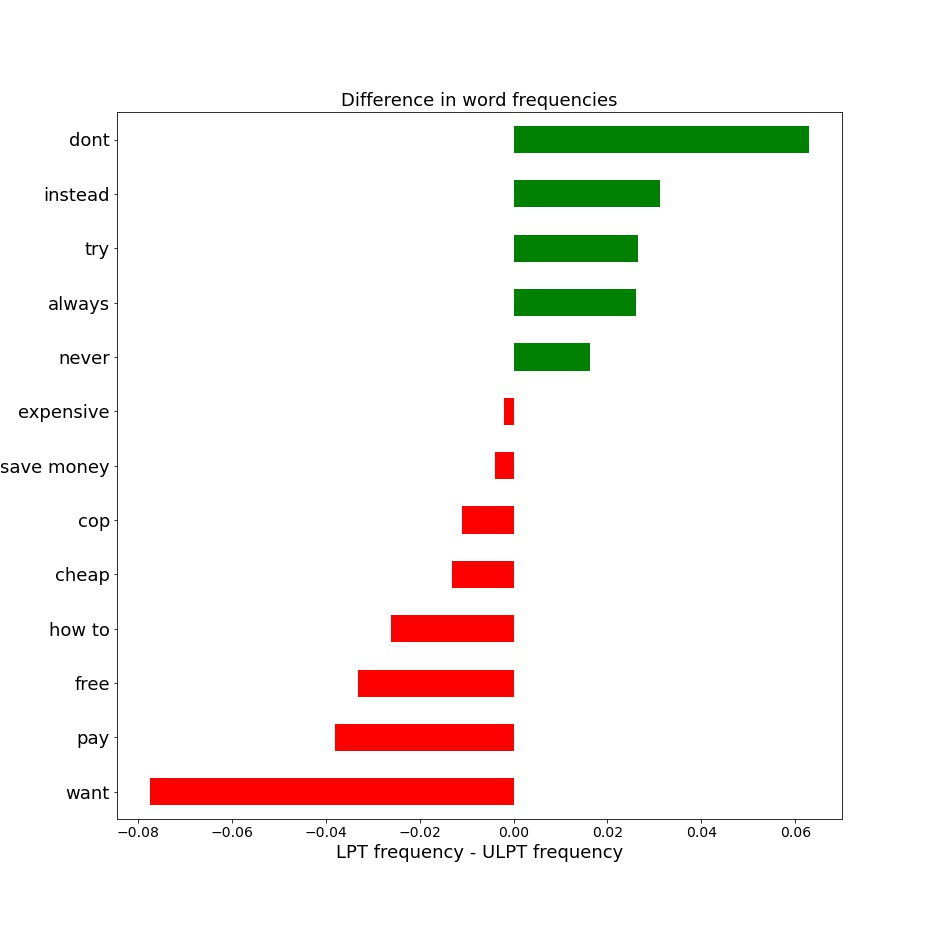
\includegraphics[width=8cm]{prelim_word_freq.jpeg}
\end{figure}

}

\frame{\frametitle{EDA: reading level}

\begin{center}
\begin{table}
\caption{Flesch-Kincaid grade levels for \texttt{title}}\label{readinglevels}
\begin{tabular}{|p{0.3\linewidth}|p{0.1\linewidth}|p{0.1\linewidth}|p{0.1\linewidth}|p{0.1\linewidth}|p{0.13\linewidth}|}
\hline
subreddit & mean & std & Q1 & median & Q3\\
\hline
LifeProTips & 7.0028 & 3.5783 & 4.5   & 6.8 & 9.1 \\
\hline
UnethicalLifeProTips & 6.3536 & 3.8397 &  3.8  & 6.0 & 8.3 \\
\hline
\end{tabular}
\end{table}
\end{center}
\vfill

}

\frame{\frametitle{EDA: reading level}

\begin{figure}
\centering
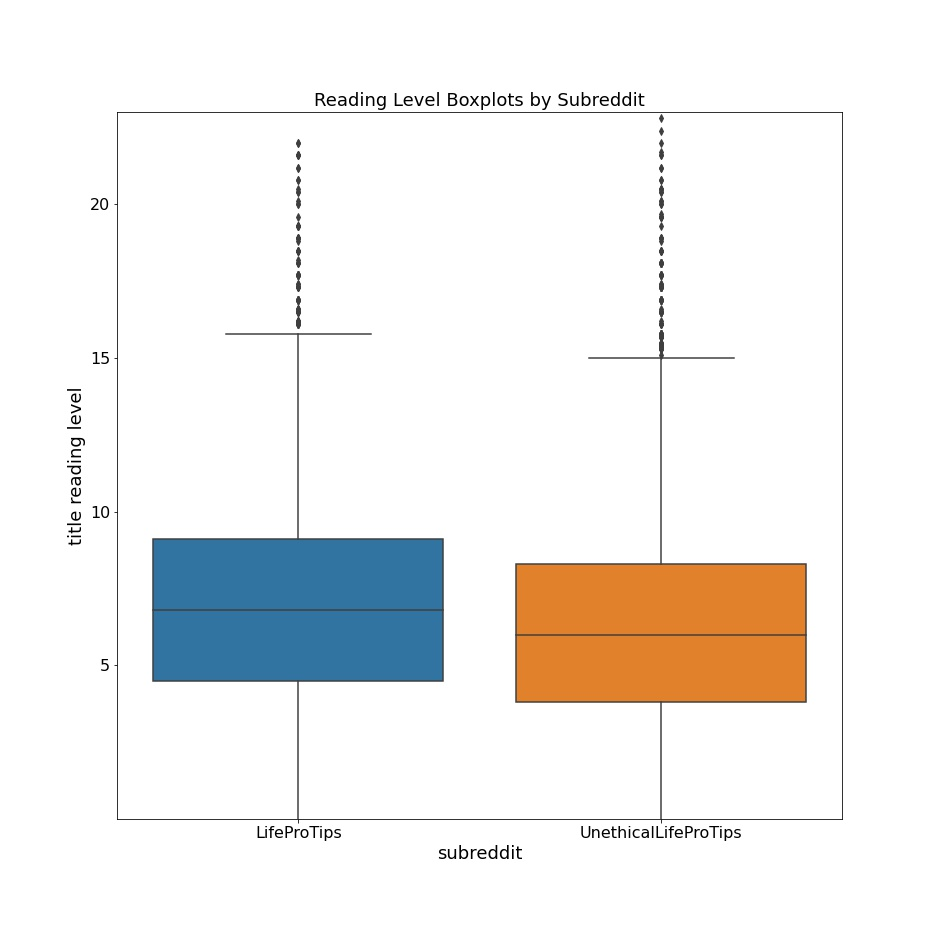
\includegraphics[width=8cm]{readinglevel_boxplot.jpeg}
\label{readinglevel_boxplot} 
\end{figure}

}


\frame{\frametitle{EDA: Clustering LPT topics}

All LPT topics align with self-improvement theme.

}

\frame{\frametitle{EDA: Clustering LPT topics}

 \textbf{Resolutions:} The data were scraped from Reddit in early January, so there were understandably a large number of recent posts addressing New Year's resolutions.  Here are some samples from this topic:

 \begin{quote}
\tql Don’t wait for the first day of the new year to start or change something. TODAY is the day to start, no matter where it falls on the calendar!\tqr
\end{quote}

\vp

 \textbf{Cooking/kitchen tips:} There was significant representation of tips and advice regarding cooking and preparing food.  Some notable samples are:

\begin{quote}
\tql Don't use the microwave to heat up pasta from the fridge, but use a frying pan and a little bit of water\tqr
\end{quote}

\vfill

}

\frame{\frametitle{EDA: Clustering LPT topics}

\textbf{Money:} Tips about money management were often clustered together.  Samples:

 \begin{quote}
\tql if you’re about to spend a good chunk of money on something you don’t really need, stop and invest the money instead.\tqr
\end{quote}

\vp

\textbf{Gift giving:} Again, because the data were scraped near the holidays, there were many posts referring to Christmas gifts.  Some samples include:

 \begin{quote}
\tql Keep an ongoing list of potential Christmas presents for your loved ones throughout the whole year. Every time they mention something they’d like to have, write it down\tqr
\end{quote}

\vfill

}

\frame{\frametitle{EDA: Clustering LPT topics}

\textbf{Mental health:} This is not a surprising topic to have received attention in the LPT subreddit.  Some examples of posts are the following:

 \begin{quote}
\tql It’s okay (and often healthy) to take a break from listening to drama and overhyped, overinflated news/opinions on social media and mainstream news stations\tqr
\end{quote}

\vp

\textbf{Cleaning:} Many tips surrounded the topic of cleaning.  Here are a few examples:

 \begin{quote}
\tql When cleaning the house, if you're bringing something from one room to another, bring back something that belongs to the room you were in.\tqr
\end{quote}

\vfill

}

\frame{\frametitle{EDA: Clustering LPT topics}

\textbf{Online behavior:} Another common theme is advice regarding online behavior: managing online profiles, accounts, passwords, etc.  Samples:

 \begin{quote}
\tql have 3 passwords: one for your main mail account, one for websites with your card info, one for the other\tqr
\end{quote}

\vfill

}

\frame{\frametitle{EDA: Clustering ULPT topics}

All ULPT topics align with the dishonesty-for-gain-from others theme.

}

\frame{\frametitle{EDA: Clustering ULPT topics}

\textbf{Avoid ads/paywalls:} This topic includes tips on how to avoid ads or paywalls on various websites.  Samples:

 \begin{quote}
\tql Press Control+A, then Control+C to highlight and copy an article before the paywall pops up. Then paste it into a Google or Word Document to read it.\tqr
\end{quote}

\vp

\textbf{Scamming return policies/rewards programs:} Another large class of ULPT posts included advice on how to exploit the return policies and rewards programs of various businesses.  Examples include:

 \begin{quote}
\tql If you need to get a new refrigerator filter, buy a new filter, then put the old filter back in the package and return it saying you bought the wrong one.\tqr
\end{quote}
\vfill

}

\frame{\frametitle{EDA: Clustering ULPT topics}

\textbf{Get out of work:} There is a lot of advice in ULPT on how to get away with doing little to no work at your job.  Examples:

\begin{quote}
\tql Working from home and need to appear online? Prop up a lock on the period button within the note pad application.\tqr
\end{quote}

\vp

\textbf{Interpersonal deception/spite/prank:} This is a broad category. Behavior including deception, eavesdropping, lying, manipulation, emotional abuse is covered by this category.  The tips in this category are less for monetary or material gain and more for spite or some sort of social/emotional/intangible advantage over another individual.  Some examples include:

\begin{quote}
\tql When you have guests over make the medicine cabinet full where if they try to open it things will fall out and you’ll hear the noise. Then you will know if they’re snooping around\tqr
\end{quote}

\vfill

}

\frame{\frametitle{EDA: Clustering ULPT topics}

\textbf{Getting something for nothing:} This topic includes advice for how to get something for free or for less than full price/effort. Samples:

\begin{quote}
\tql If shipping packages through USPS, use the self service checkout and when you weigh your item, lift the corner of your package off the scale for a cheaper shipping rate\tqr
\end{quote}

\vp

\textbf{Car related:} There is also a large representation of advice regarding getting out of traffic/parking violations and similar situations.  Examples:

\begin{quote}
\tql Pass a cop while speeding on the highway and they start turning around to pull you over? Call 911 and report a drunk driver a few miles behind you.\tqr
\end{quote}

\vfill

}



\frame{\frametitle{EDA: Most predictive title words for LPT}

\begin{figure}
\centering
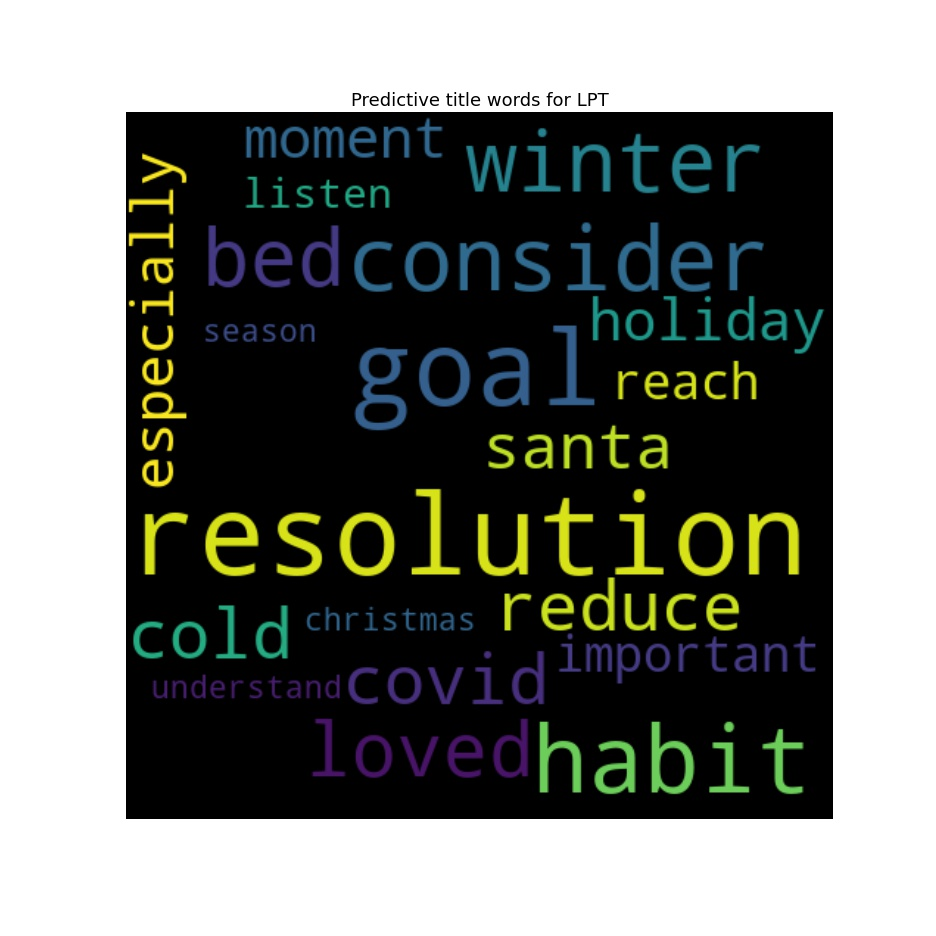
\includegraphics[width=8cm]{LPT_title_wordcloud.jpeg}
\end{figure}
}

\frame{\frametitle{EDA: Most predictive title words for ULPT}

\begin{figure}
\centering
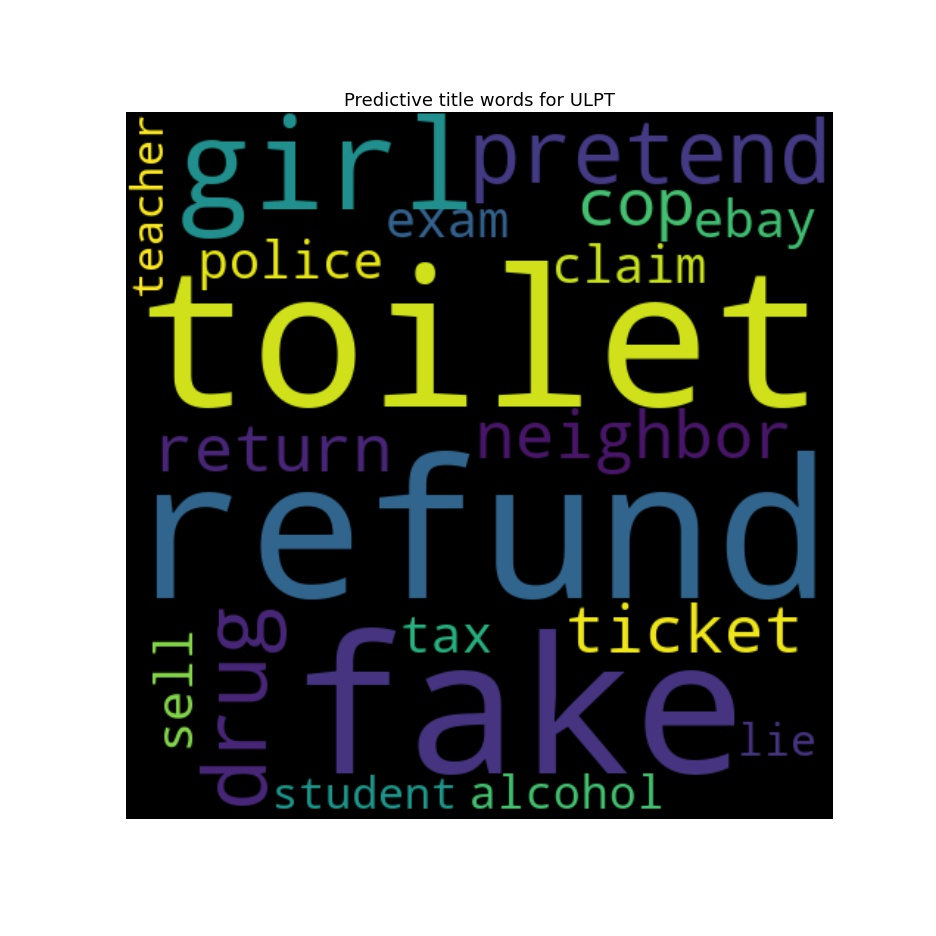
\includegraphics[width=8cm]{ULPT_title_wordcloud.jpeg}
\end{figure}
}

\frame{\frametitle{Model selection}
\pause
\begin{table}
\caption{Cross-validation results}
\begin{tabular}{|p{0.25\linewidth}|p{0.35\linewidth}|p{0.1\linewidth}|p{0.1\linewidth}|}
\hline
Estimator & Hyperparameters & Mean CV Accuracy & Test Accuracy\\
\hline
\texttt{RandomForest}-\texttt{Classifier} & \texttt{criterion='gini', max\_depth=78, max\_features='log2', n\_estimators=143} & 0.7614 & 0.7880\\
\hline
\texttt{MultinomialNB} & \texttt{alpha=1} & 0.7772 &0.7917 \\
\hline
\texttt{Logistic}-\texttt{Regression} & \texttt{C=0.1, dual=False, penalty='l2', tol=0.0001} & 0.7714 & 0.8022\\
\hline
\end{tabular}
\end{table}
}

\frame{\frametitle{Threshold tuning}

Unethical advice filter: emphasize precision. 
\vp
Selected model: \texttt{RandomForestClassifier} with threshold 0.5718.
\vp
Positive precision: 89.03\%
\vp
Positive recall: 50.2\%
\vfill
}

\frame{\frametitle{Precision-recall curve}

\begin{figure}
\centering
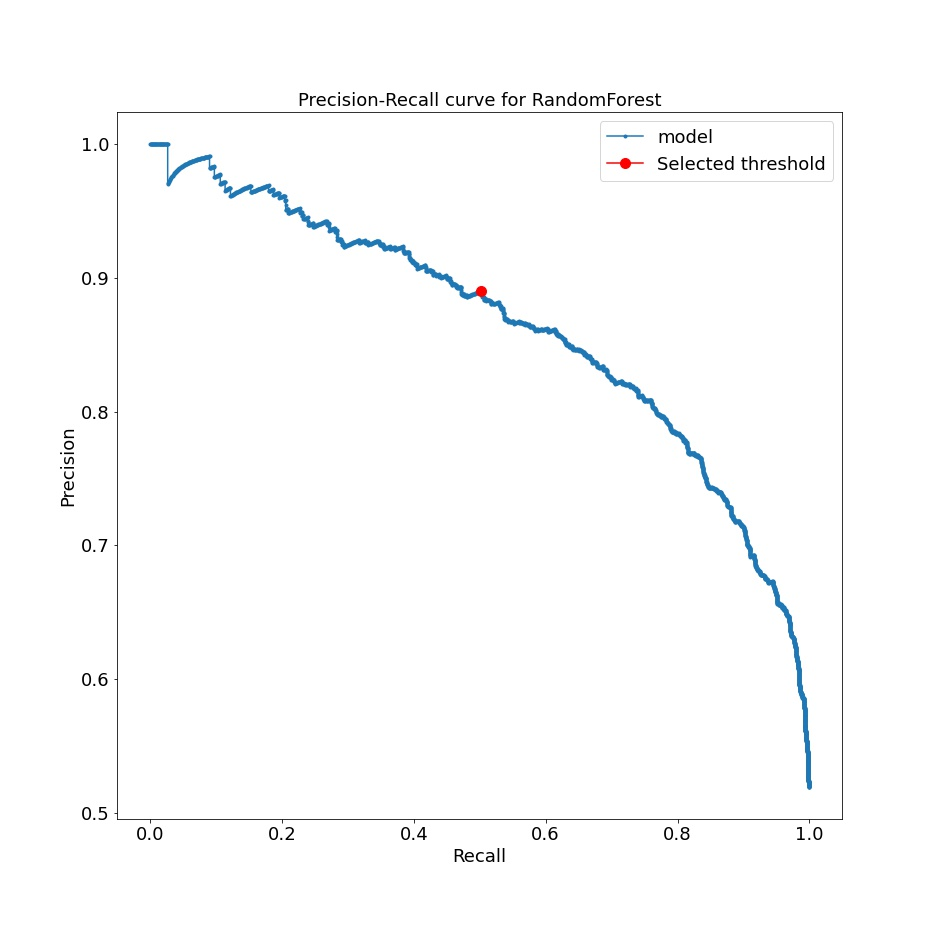
\includegraphics[width=8cm]{RF_precision_recall.jpeg}
\end{figure}

}

\frame{\frametitle{Confusion matrix}

\begin{table}
\caption{Confusion matrix for \texttt{RandomForestClassifier} with threshold 0.5718 predicting ULPT}\label{RF_cm}
\[\begin{array}{|c|c|c|}
\hline
& \text{Predicted False} & \text{Predicted True}\\
\hline
\text{Actual False} & 47.0\% & 3.2\%\\
\hline
\text{Actual True} & 24.6\% & 25.2\%\\
\hline
\end{array}\]
\end{table}

}




\frame{\frametitle{Summary}

\begin{itemize}

\item Use: automatically detect unethical advice
\vp

\item Precision: 89.03\%
\vp

\item Recall: 50.20\%
\vp


\end{itemize}

}


\frame{\frametitle{Next steps}

\begin{itemize}

\item Use more data
\vp

\item Automate collection and training
\vfill

\end{itemize}

}

\end{document}
